% Technické detaily učení z preferencí (RLHF s PPO, DPO), dříve součást llms.tex

% ----------------------------------------------------------------------------

\begin{frame}{Zpětnovazebné učení}

    \centering
    \begin{tikzpicture}

        \node (prompt) {Prompt from dataset/logs};

        \node[inner sep=5pt,fill=ufallightblue, below=40pt of prompt,minimum height=50pt] (lm) {\begin{minipage}{100pt}\centering\large Language \\ model \end{minipage}};

        \draw[->] (prompt) -- (lm);

        \node[below=40pt of lm] (answer) {Sampled answer};

        \draw[->] (lm) -- (answer);

        \visible<2->{
        \node[inner sep=5pt,fill=ufalgreen, right=130pt of lm,minimum height=30pt] (reward) {\begin{minipage}{80pt}\centering Reward \\ model \end{minipage}};
        \draw[->] (answer.east) to[out=0,in=270, looseness=0.7] (reward.south);
        \draw[->] (prompt.east) to[out=0,in=90, looseness=0.7] (reward.north);
        }

        \visible<3->{
        \node[right=40pt of lm,fill=ufal,circle] (optim) {\begin{minipage}{40pt}\centering Proximal \\ Policy \\ Optim. \end{minipage}};
        \draw[->] (reward) -- (optim);
        \draw[->] (optim) -- (lm);
        }

    \end{tikzpicture}

\end{frame}

% ----------------------------------------------------------------------------

\begin{frame}{Direct Preference Optimization}

    \centering
    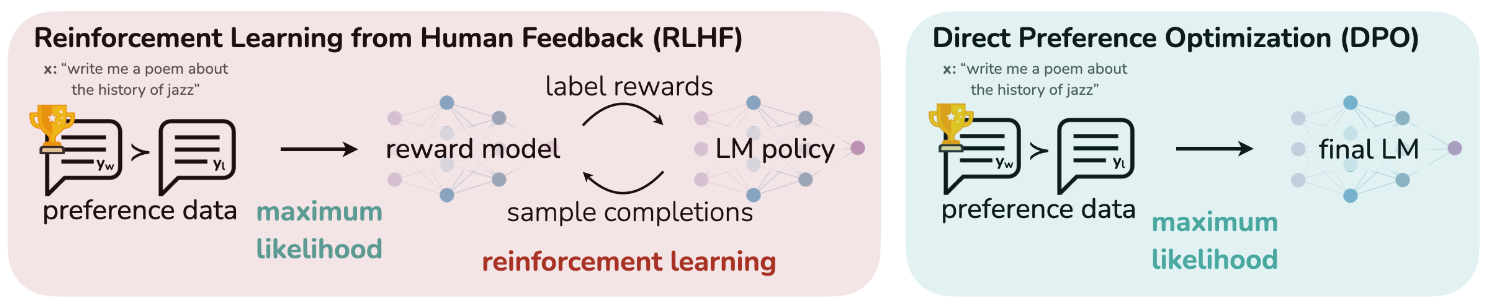
\includegraphics[width=.9\textwidth]{img/dpo.png} \\[1em]
    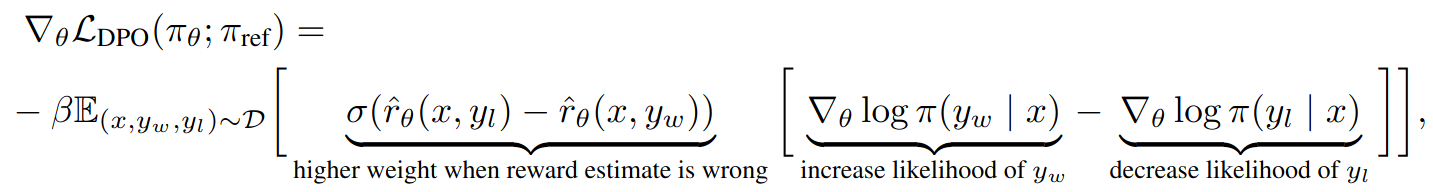
\includegraphics[width=.9\textwidth]{img/dpo-equation.png} \\

    \tiny Zdroj: \citet{rafailov2024direct}

\end{frame}
